\documentclass[10pt]{beamer}
\usetheme{Warsaw}
\usepackage[utf8]{inputenc}
\usepackage[english]{babel}
\usepackage{amsmath}
\usepackage{amsfonts}
\usepackage{amssymb}
\usepackage{graphicx}
\setbeamersize{text margin left=0.3cm,text margin right=0.3cm} 

\graphicspath{ {../figures/} }

\usepackage[style=authortitle,doi=false,isbn=false,url=false,backend=bibtex]{biblatex}
\addbibresource{../bvitali_biblio}

%%%%NO_IDEA-BUT_IMPORTANT%%%%
\usepackage{sansmathaccent}
\pdfmapfile{+sansmathaccent.map}
%%%%%%%%%%%%%%%%%%%%%%%%%%%%%

\author[Bastiano Vitali]{{\Large Bastiano Vitali}\\\ \\{\small Prof. Simone Donati (INFN, UniPi)\\ Dr. Pavel Murat (FNAL)}}
\title{In situ monitoring of the stopped muon flux at Mu2e}
%\setbeamercovered{transparent} 
%\setbeamertemplate{navigation symbols}{} 
\titlegraphic{
\includegraphics[scale=0.7]{cherubino.jpg}\ \ 
\includegraphics[scale=0.065]{mu2e_logo}}%%\institute{} 
\date{} 
%\subject{} 

\makeatother
\setbeamertemplate{footline}
{
  \leavevmode%
  \hbox{%
  \begin{beamercolorbox}[wd=.4\paperwidth,ht=2.25ex,dp=1ex,center]{author in head/foot}%
    \usebeamerfont{author in head/foot}\insertshortauthor
  \end{beamercolorbox}%
  \begin{beamercolorbox}[wd=.6\paperwidth,ht=2.25ex,dp=1ex,center]{title in head/foot}%
    \usebeamerfont{title in head/foot}\insertshorttitle\hspace*{3em}
    \insertframenumber{} / \inserttotalframenumber\hspace*{1ex}
  \end{beamercolorbox}}%
  \vskip0pt%
}
\makeatletter
\setbeamertemplate{navigation symbols}{}

\begin{document}

\begin{frame}
\titlepage
\end{frame}

\begin{frame}{Mu2e experiment}
\begin{itemize}
\item After $\nu$ oscillations \footcite{signorelli}, is Charged Lepton Flavour Violation possible?\\
\item Mu2e looks for $\mu\rightarrow e$ conversion (near Al$^{27}$ nucleus)
\begin{itemize}
\item SINDRUM II set the limit at $7\times 10^{-13}$ and Mu2e aims at $\mathcal{O}(10^{-17})$
\item The signal is a monoenergetic electron of $ \approx 104.97$ MeV
\end{itemize}
\begin{figure}
\centering
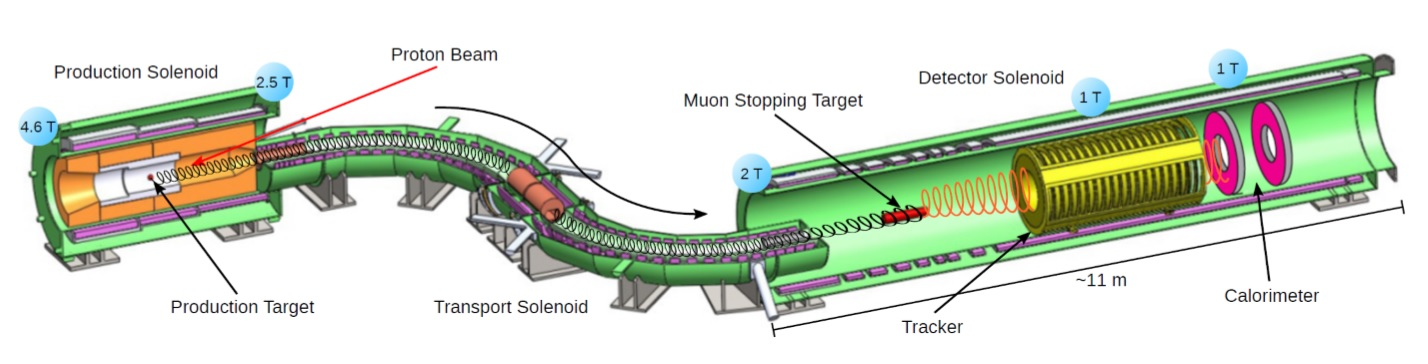
\includegraphics[width=0.8\textwidth]{mu2e_apparatus}
\caption{Mu2e apparatus: $\mu$ stopped in Al target; straw-tube tracker in yellow}
\end{figure}
\end{itemize}
\end{frame}

\begin{frame}{Stopped muon flux monitor}
\begin{itemize}
\item Resonant extraction: beam intensity variations on a 1 ms scale
\item Physical processes
\begin{itemize}
\item Deexcitation of muonic atoms $\rightarrow$ HPGe and LaBr$_3$ \hfill [Too low rate]
\item Nuclear muon capture $\rightarrow$ ejected proton counting \hfill [2k/1.7 $\mu$s]
\begin{itemize}
\item high energy deposition in the tracker ($\sim 1/\beta^2$) 
\item higher multiple scattering ($\sim 1/\beta p$)
\item absorbers $\rightarrow$ higher momenta than electrons
\end{itemize}
\end{itemize}
\end{itemize}   
\begin{figure}
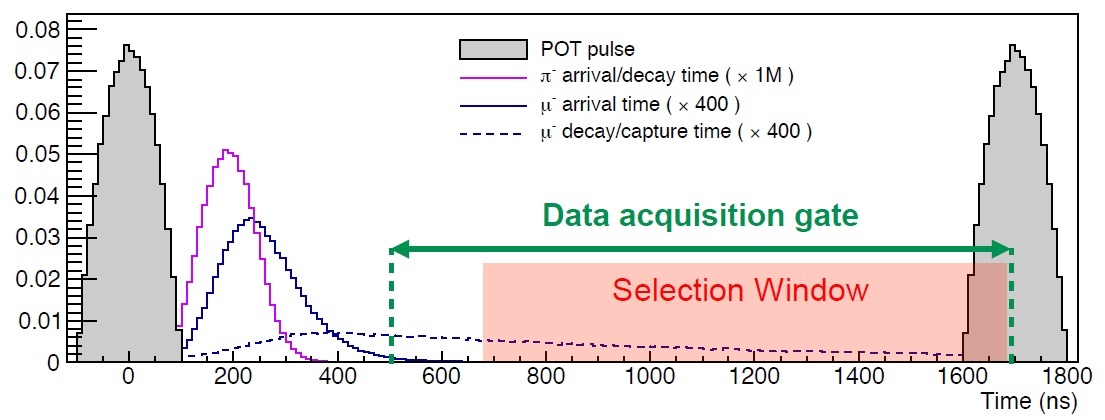
\includegraphics[width=0.8\textwidth]{mu2e_event}
\caption{Mu2e \textit{event}: everything between two proton pulses}
\end{figure} 
\end{frame}

\begin{frame}{Some key features}
\begin{itemize}
\item Most of the work done was code related and 'less then engaging'...
\item The the most intriguing studies
\begin{itemize}
\item Possible cuts on the deposited charge in the straws
\item Topology of the tracks
\end{itemize} 
\end{itemize}
\begin{figure}
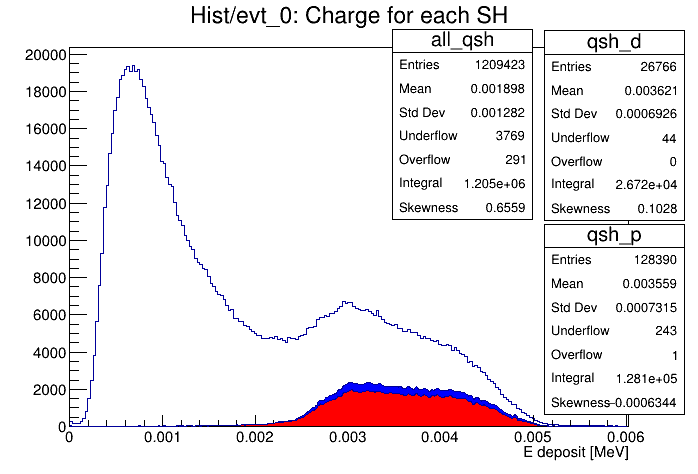
\includegraphics[height=4cm]{plots/mix/mix500_qsh}%
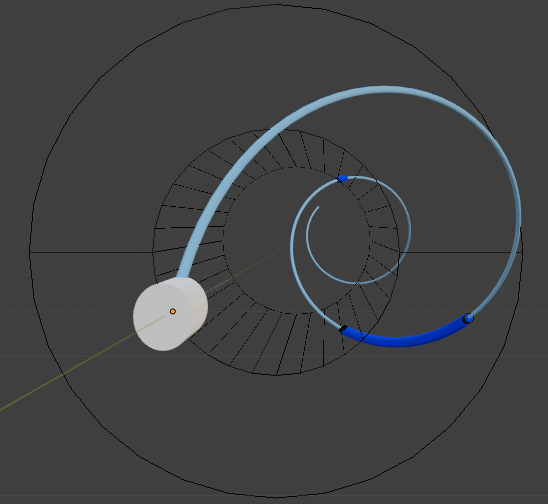
\includegraphics[height=4cm]{Blender_Tracker_4}%
\caption{Energy deposit in the straws and tricky topology}
\end{figure}
\end{frame}



\begin{frame}{Single particle efficiency}
\begin{figure}
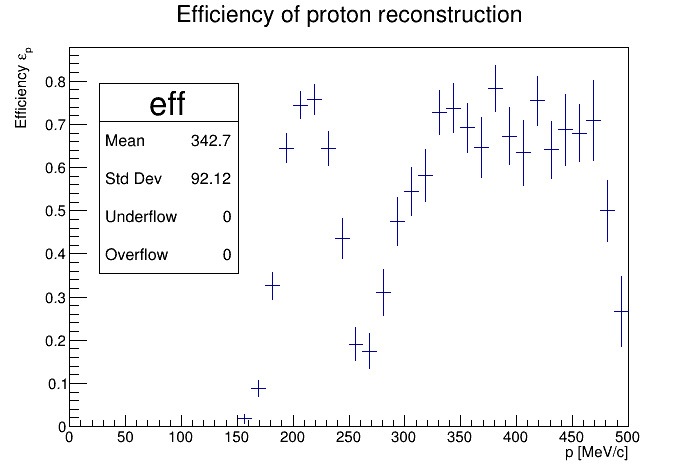
\includegraphics[scale=0.4]{Report_3/pgun2_SHminE0_L_eff_genp3}
\caption{Reconstructed/particles with at least 1 hit in the tracker}
\end{figure}
\end{frame}

\begin{frame}{Conclusions}
\centering
Number of tracks $\approx 4.5/1.7\ \mu$s\\\textbf{Adequate for monitoring fluctuations on ms}
\begin{figure}
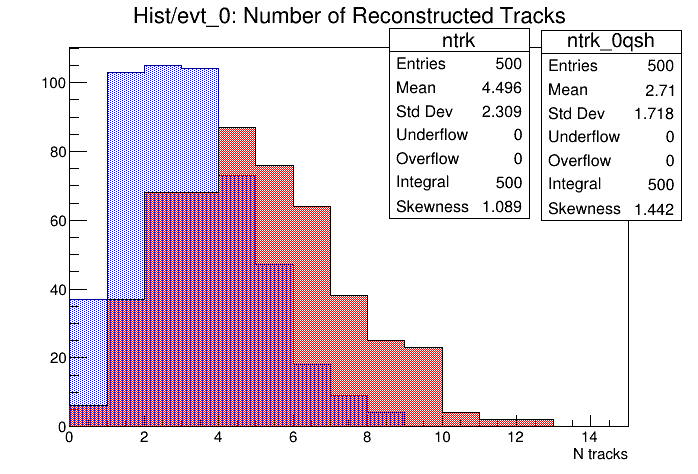
\includegraphics[scale=0.38]{plots/mix/mix500_trk}
\caption{The number of reconstructed tracks per event (red: cut on SH energy)}
\end{figure}
\end{frame}

\begin{frame}{Backup: Tracker}
\centering
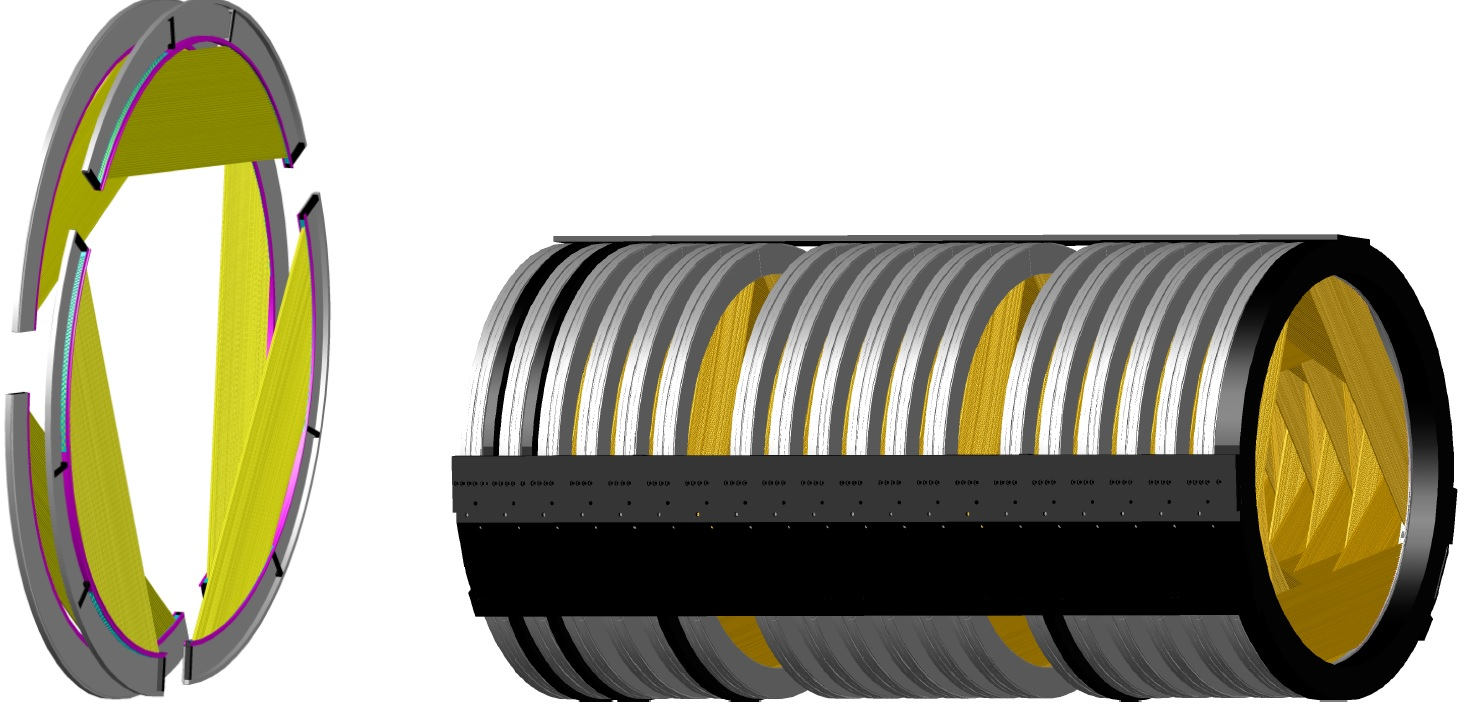
\includegraphics[scale=0.4]{mu2e_tracker}
\end{frame}

\begin{frame}{Backup: Spectra parameterizations}
\centering
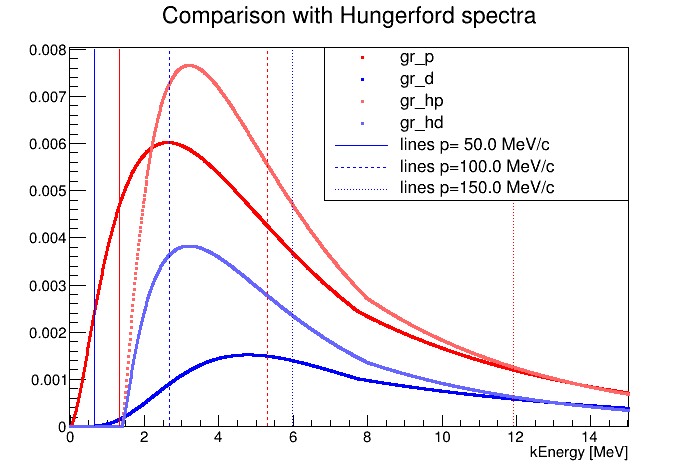
\includegraphics[scale=0.45]{/new_spectra_2/comparison2}
\end{frame}

\begin{frame}{Backup: Reconstructed momentum}
\centering
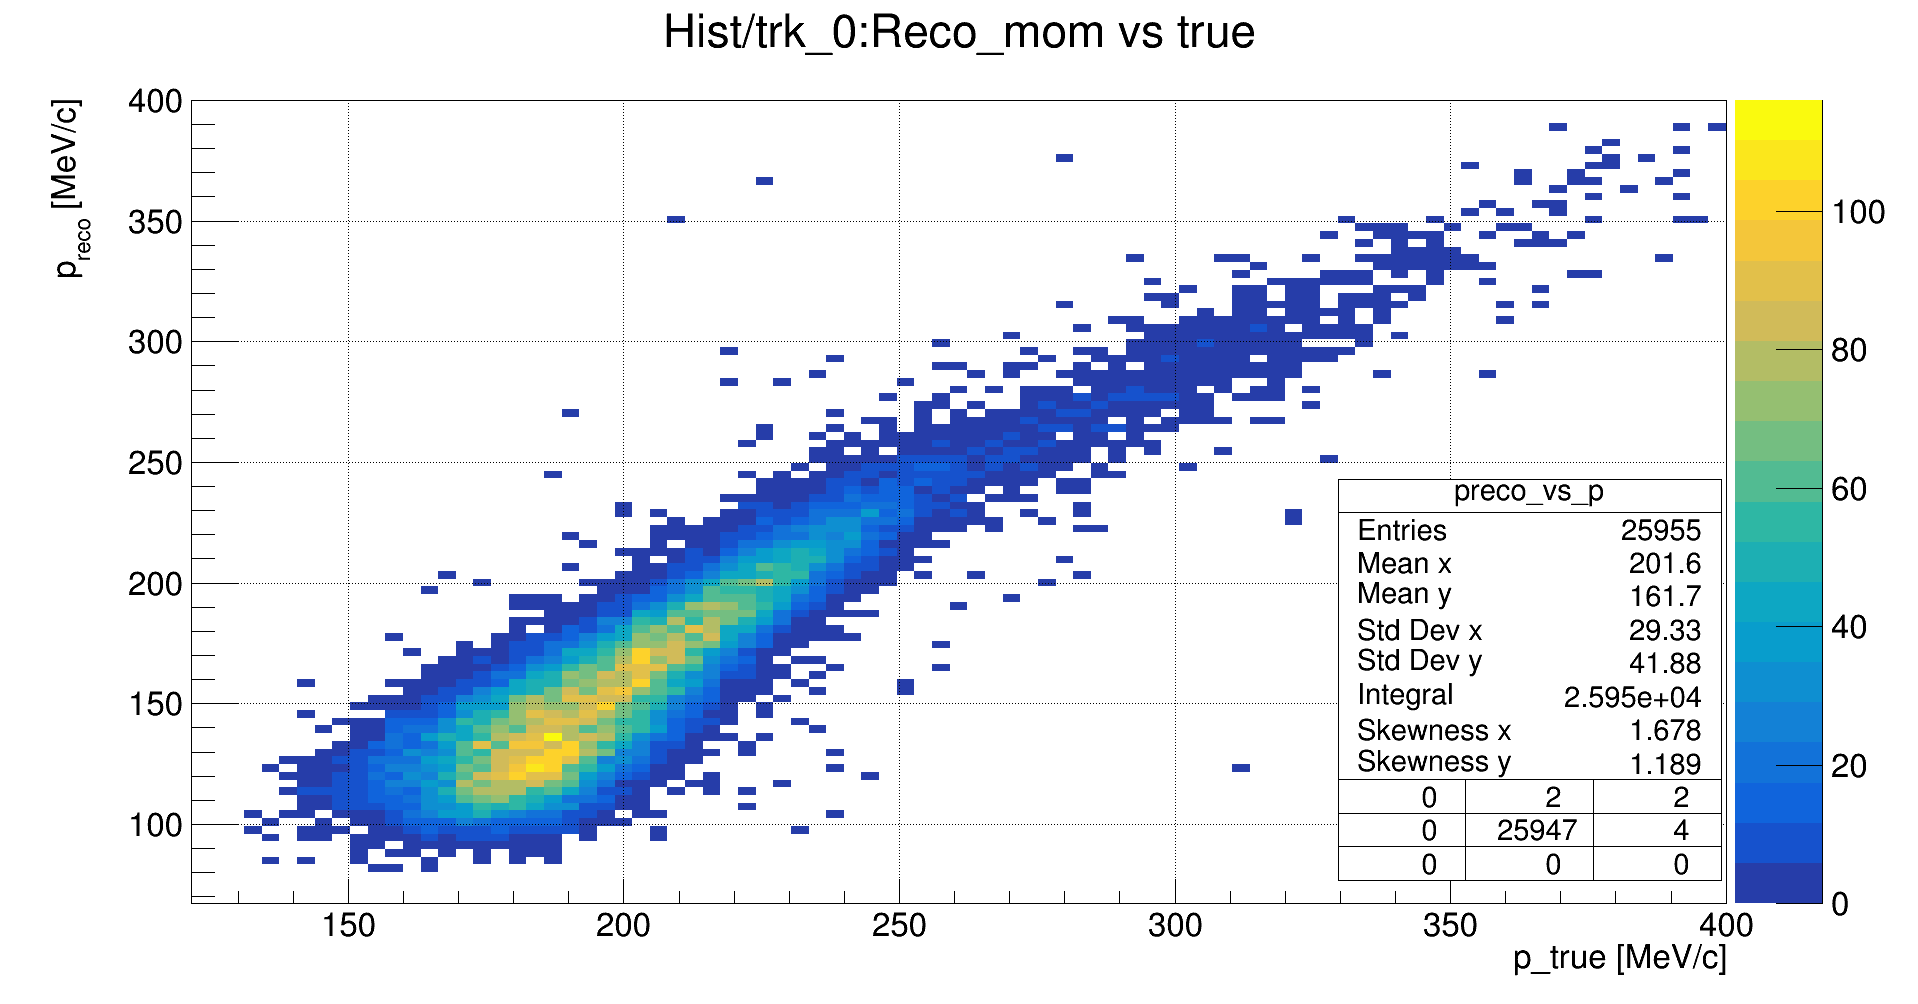
\includegraphics[width=\textwidth]{FR/PrecoVsP}
\end{frame}

\begin{frame}{Backup: Software structure}
\centering
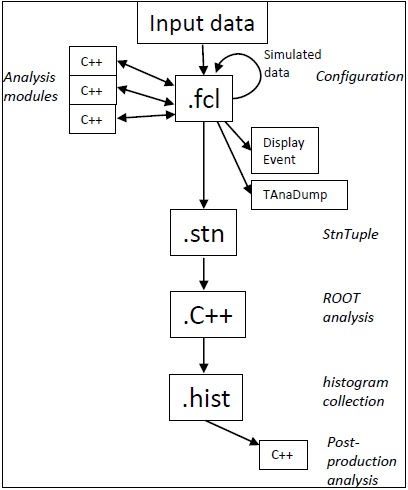
\includegraphics[height=0.8\textheight]{mu2e_datahandling}
\end{frame}

\setbeamertemplate{bibliography item}{}

\begin{frame}
\printbibliography
\end{frame}

\end{document}

%%%%%%%%%%%%%%%%%%%%%%%%%%%%%%%%%%%%%%%%%%%%%%%%
\begin{itemize}
\item After $\nu$ oscillation, Charged Lepton Flavour Violation is an open question
\item Mu2e looks for $\mu\rightarrow e$ conversion (near Al$^{27}$ nucleus)
\begin{itemize}
\item In the SM, depends on $\Delta m_{\nu}^2 \rightarrow$ BR$\approx10^{-54}$
\item Many theories, SUSY among them, predict higher BR
\item The aim is Single Event Sensitivity of $10^{-17}$
\end{itemize}
\begin{figure}
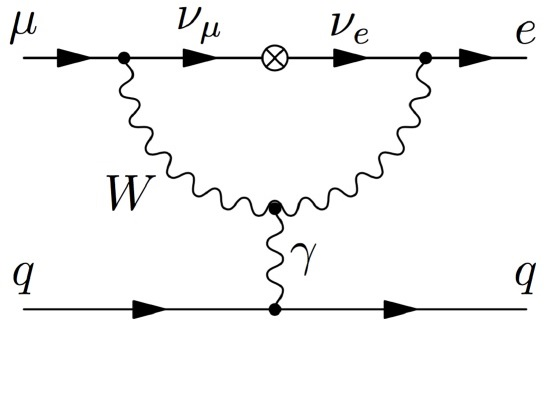
\includegraphics[scale=0.4]{feynman_mu2e}
\caption{SM Feynman diagram of $\mu\rightarrow e$ conversion}
\end{figure}
\end{itemize}

\begin{center}
\resizebox{.9\textwidth}{!}{%
\includegraphics[height=3cm]{example-image-a}%
\quad
\includegraphics[height=3cm]{example-image-16x9}%
}
\end{center}